%%%%%%%%%%%%%%%%%%%%%%%%%%%%%%%% 
\section{The Field Cage and High Voltage System} 
\label{sec:detectors-fd-alt-hv}

This section describes the design of the high voltage system, field
cage and cathode for the TPC.  It is taken from the 
%A detailed description of the design of the HV system, field cage andcathode for the 
LBNO 20-kt and 50-kt detector design, described in \anxlbnoa and \anxlbnob,
% is provided in the deliverable document 3.1 (LAr experiment) of the LAGUNA-LBNO design study\cite{LAGUNA-LBNO-deliv}. 
and can be simplified and down-sized for the DUNE detector 
(12~kt or 15~kt), % detectors with some simplifications and down-sizing
due to the shorter drift path and the rectangular aspect ratio of the
detector. The much shorter transversal dimension of DUNE with respect to the LBNO design
permits a lighter cathode structure (less sag requires less compensation) 
%to be compensated with respect to the octagonal detector) 
and a simpler hanging system for the drift cage and the cathode.

The field cage in this design is
composed of equally spaced octagonal rings that create a uniform
drift field of 500--1000~V/cm. This leads to a cathode voltage of up to 2~MV 
%at the cathode is needed 
to provide a drift field at
the maximal intensity of 1~kV/cm over a drift distance of 20~m. \fixme{drift field intensity maximal
with respect to time or space? I don't understand}

Two different approaches have been developed %considered and realized 
for the
drift-field HV system. The first approach uses an external HV power supply
and uses HV feedthroughs to penetrate into the detector volume.
%feeds it \fixme{feeds the voltage} into the detector volume using HV feedthroughs. 
The  WA105 demonstrator will use this
approach %is going to be applied in the WA105 demonstrator 
for its drift
of 6~m and a cathode voltage up to 600~kV.  The second approach is
based on a HV generator directly inside the LAr volume, \fixme{which is the} same
as the Greinacher HV multiplier. It is an innovative technique, 
%to generate a HV for creating a drift electric field in a LArTPC, 
with
some advantages relative to the first approach. This technique
particularly suits giant-scale detectors that require a very high voltage of
$\sim$1--2~MV. The DUNE detector (12-m drift) requires a voltage
of 600~kV  in order to operate at a field intensity of
0.5~kV/cm. This voltage is a factor of 3.3 higher than that for %the one foreseen in 
the reference design (Chapter~\ref{ch:fd-ref}) and it is in the scope of the WA105 detector
operation at 1~kV/cm over a 6-m drift. \fixme{this voltage will be tested in WA105?}

The field cage designed for the LBNO 20-kt detector (20-m drift
path) is composed of 99 octagonal field-shaping coils manufactured
from 316L stainless-steel tubing \fixme{and long radius elbows to EN 10217-7
shop using a combination of welded and clamped joints. (I can't parse this)} 
The coils are supported by 32 off-hanging columns of G-10CR
glass fibre/epoxy-laminated sheet insulating material, built in the form of chains and suspended from the tank deck structure. % by a special hanging support system.
Each  coil is designed as a series of fully welded infill tubes intended to
fit between \fixme{a pair of?} hanging support columns to form one section of the field cage.  Short sections
of the field-shaping coils are integrated as pins into links to assemble each
chain.  Longer sections and 
corner sections of the field-shaping coil are then fixed between the hanging columns to complete
each coil (Figure~\ref{fig:LBNO_FC}). The combined assembly of 99 sets  %%%%%%%%%%%%
of field shaping coils within the 32 off-hanging columns provides
a complete field cage.
\begin{cdrfigure}[Assembly concept of the field cage]{LBNO_FC}
{\small Left: assembly of the elements of a hanging chain. Right: 
construction of a field cage section from the hanging chains and the field shaping coil elements.}
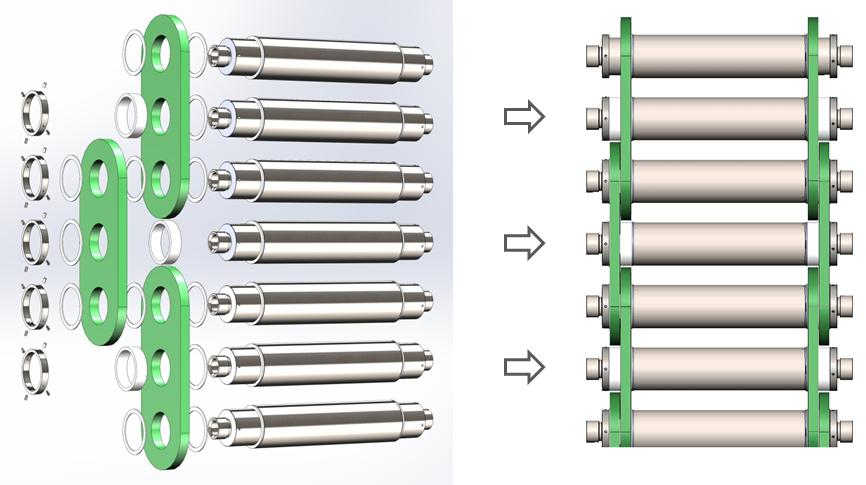
\includegraphics[width=.5\linewidth]{LBNO_chains} \hfill
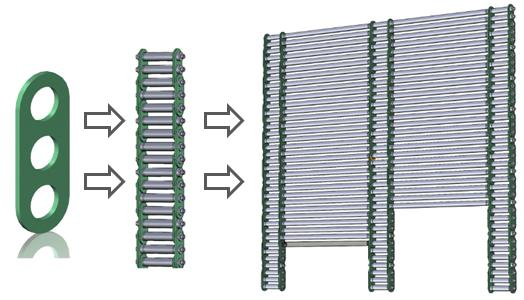
\includegraphics[width=.4\linewidth]{LBNO_FC2}
\end{cdrfigure}

The infill tube specifications assume %foresee 
an outer diameter of 139.7~mm, which
is common to the cathode structure. %but 
This allows a thinner wall, 1.6~mm, % section  
to be used %where required 
in non-structural parts of the %field shaping
coils.  Although a non-standard size, the total length of the %1.6-mm wall-thickness 
tube %required for the field shaping coils 
can be
manufactured as a special mill run. % Using this approach it will be
This will make it possible to save 21~tons of material relative to the standard tubes
(wall thickness of 2.0~mm). The wall thickness of the link pins 
is 2.6~mm; this will provide sufficient \fixme{section modulus to react the
bending moments across the link pins. (maybe ok, but I don't understand the terms.)} All specialist preparation and
welding of the link pins will be carried out in shop facilities under controlled
fabrication.  This includes the rough machining
of the end fittings, preparation of the tube ends and the jig-welding
of the complete assemblies. Further machining %, after welding 
will be
carried out to ensure correct alignment and tolerance levels in
conjunction with the hanging columns.  Vent holes will be incorporated
into the tubes as required to facilitate construction and to allow
purging with GAr/LAr on commissioning.

Manufacturing, transportation and construction considerations were a fundamental
part of the field-shaping coil design process, in
collaboration with the LAGUNA-LBNO industrial partners.
%A fundamental part of the field-shaping coil design process, in collaboration with the LAGUNA-LBNO industrial partners, involved the consideration of how such tubes could be manufactured to a high level of accuracy, transported to site, moved underground and then 
The requirement of construction in a clean-room environment within the completed membrane tank
 presented considerable challenges in
terms of logistics and the development of the overall concept for
fabrication.  It was concluded that a modular construction approach
would be required in order to  (1) maximize off-site shop fabrication and
minimize on-site assembly, %.  This approach was also considered essential in order to
and (2) ensure the cleanliness of construction and to
minimize the installation time. 
\fixme{The following is not clear to me. Here's what I think it means:
Each coil is composed of three pieces. The same pieces are used in the coils as in the cathode
structure, but the pieces are assembled differently. Am I close?}
The breakdown of each field-shaping
coil is made into sets of three main modules.  Although separate modules,
the field shaping coils and the cathode structure share identical
features and dimensions.  Thus, the maintenance of common interfaces
is an important advantage %forms an essential part 
of the overall %detector 
field cage design. %The field cage design for 
The DUNE  12-kt detector field cage would %, is based on the same concept developed for LBNO, 
include 60 rectangular rings used to cover the
12~m of drift volume.

The LBNO cathode design for the 50-kt detector %developed following 
follows an extensive
review of options and analysis.% to optimize the design for the specific requirements of the 50~kt LAr Detector.  
The design incorporates
features to minimize the static deflection of the cathode and to
maximize the electrostatic performance. (To avoid regions with high
electric fields, the electric field is limited to 50~kV/cm.) 
Similar to the field-shaping coil, and for the same reasons, the cathode is designed as a modular structure. 
%for maximum off-site shop fabrication and minimum on-site assembly in
%order the ensure cleanliness of construction, by using the cryostat ad
%clean room for the assembly, and 
Modular construction will also minimize the installation time. 
The cathode is designed as a fully welded tubular rectangular
(square) \fixme{the whole cathode is a rectangle but the grid is in squares?} grid structure in 2~m$\times$2~m bays, 1~m deep \fixme{deep in what dimension?} supported only from
the %outer 
periphery (Figure~\ref{fig:LBNO_cathode}).  
\begin{cdrfigure}[Cathode design]{LBNO_cathode}
{\small Left: cathode plane design for the LBNO detector. Right: breakdown of 
the cathode structure in construction modules.}
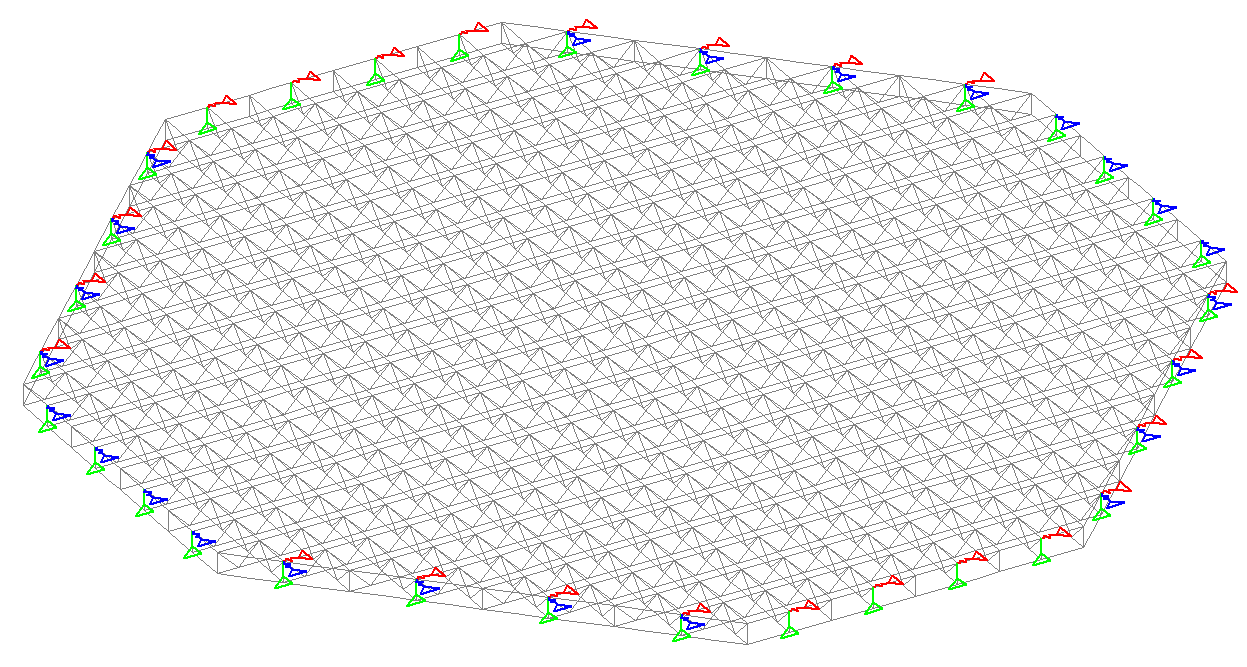
\includegraphics[width=.4\linewidth]{LBNO_cathode} \hfil
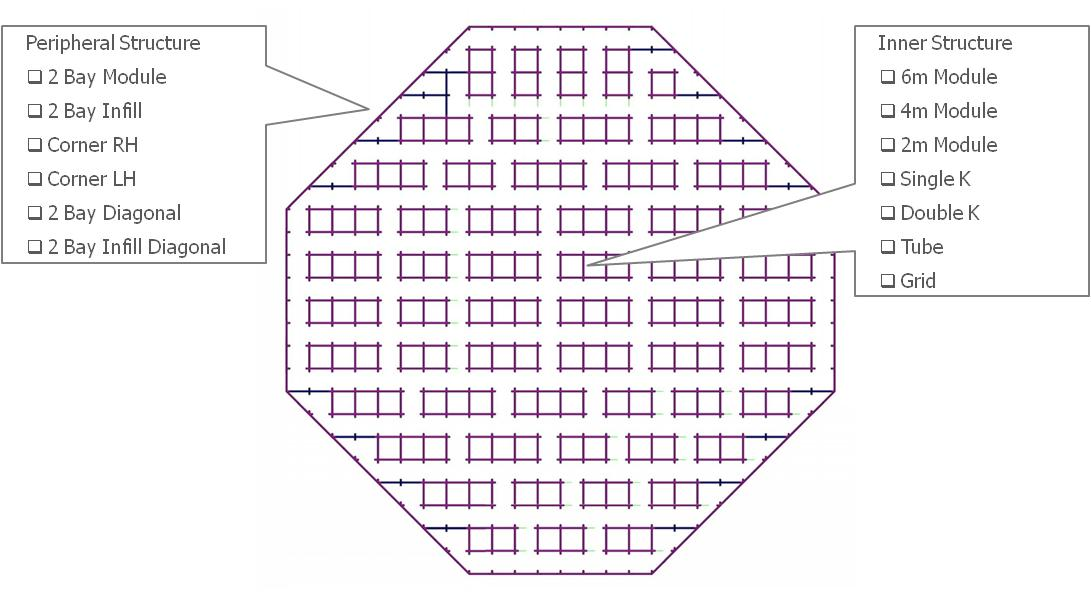
\includegraphics[width=.5\linewidth]{LBNO_cathode_elements}
\end{cdrfigure}
The top and bottom grid structures \fixme{I don't see two; are there two layers of grids in the cathode?} are manufactured from 139.7-mm OD tubes with wall thickness 
2.6~mm %wall tubes 
to EN 10217-7 \fixme{Is this a standard?} in 316 stainless steel.  The bracing
structure is manufactured from 60.3-mm OD tubes with wall thickness 2.6~mm, also to EN
10217-7 in 316 stainless steel.  A grid structure comprising 
 10-mm OD tubes with wall thickness 1~mm,
 arranged in a parallel single plane \fixme{parallel to other grid?} at 100-mm centers,
will be fitted to the top of the cathode only. \fixme{What is its function?} The maximum module size
for this structure
is 6~m, comprising three full 2~m$\times$2~m$\times$1~m deep bays
of the cathode structure.  All specialist node \fixme{node? attachment points?} preparation and welding
of the modules will be carried out in controlled facilities at the fabrication shop. 
 Vent holes are incorporated into the structures to
facilitate construction and to allow purging with GAr/LAr on
commissioning. High levels of quality control will be possible with
the modular construction design, and following inspection, each module
will be cleaned to ISO 8 cleanliness standard and double-wrapped prior
to dispatch and transportation to the site for installation and final
assembly. % of the cathode. 
The complete assembly procedure, logistics and
tooling for the field cage and cathode is described in \anxlbnob.
\fixme{Add: It is expected that these elements would be the same for the DUNE detector . }

The cathode outer top tubular structure is identical to the bottom
field-shaping coil; they use tubes of the same outer diameter
(139.7~mm).  The spans are the same (48~m for the 50-kt LBNO detector)
and the vertical distance separating these components is the same as for
the remaining field-shaping coils (200-mm centers). The cathode will be
attached at the bottom of each hanging column by a split link in
G-10CR. The cathode attachment points will also incorporate locally
thickened sections of tube (as in the hanging chains) included as part
of the peripheral structure nodes.


\fixme{already said} The cathode structure for the 12-kt DUNE far detector follows the ...
%same design concepts as the one studied for LBNO with a down-sizing of
%the elements since is is not needed to limit sagging effects over 48~m
%span but on only 12~m. This translates in a lighter and cheaper
%structure.
